\chapter{Hidrodinámica y Oscilaciones Estelares}

\noindent Buena parte de la astrofísica estelar se sustenta bajo las ecuaciones de la hidrodinámica. Es la base matemática ideal para describir el gas del interior de las estrellas como un fluido continuo. En este capítulo, dichas ecuaciones se presentan, así como su formulación en el marco de la teoría de perturbaciones.

\section{Ecuaciones Básicas de la Hidrodinámica}
Las propiedades esenciales del gas estelar pueden especificarse como funciones de la posición y del tiempo. Estas propiedades incluyen la densidad local $\rho(\mathbf{r},t)$, la presión $p(\mathbf{r},t)$, la temperatura $T(\mathbf{r},t)$ (y/o cualquier otra cantidad termodinámica relevante) y la velocidad del fluido $\mathbf{v}(\mathbf{r},t)$. Aquí, $\mathbf{r}$ denota el vector posición con respecto a un punto de referencia en el espacio, correspondiéndose con lo que vería un observador en reposo. Esta descripción, pues, se conoce como la descripción \textit{Euleriana} del fluido. Otra descripción posible es la \textit{Lagrangiana}, en la cual un observador sigue el movimiento de un elemento de fluido a medida que se desplaza por el espacio. En este marco, un elemento de gas puede ser etiquetado por su posición inicial $\mathbf{r}_0$, y sus propiedades se describen como funciones de $\mathbf{r}_0$ y del tiempo $t$ (por ejemplo, $\mathbf{r}(\mathbf{r}_0,t)$).

\begin{figure}[htbp]
    \centering
    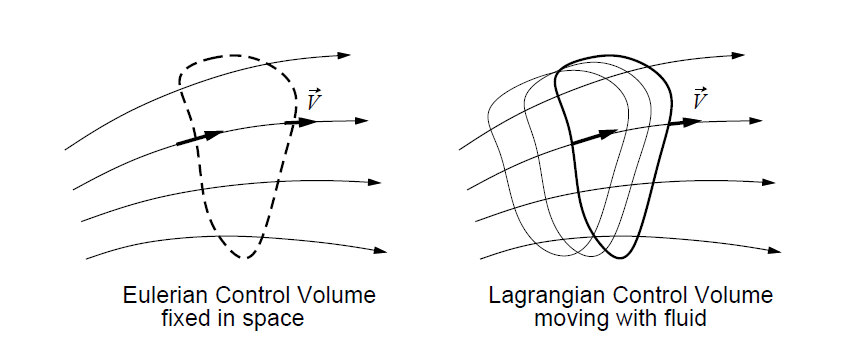
\includegraphics[width=\linewidth]{Imagenes/euler_vs_lagrange.png}
    \caption{La descripción Euleriana describe el flujo del fluido desde la perspectiva de un volumen fijo en el espacio. La descripción Lagrangiana describe el flujo del fluido desde la perspectiva de un elemento de fluido individual. Imagen tomada de \autocite{PhysicsStackExchange537111}}
\end{figure}

La derivada temporal de una cantidad $\phi$, observada desde un marco lagrangiano, es

\begin{equation}
\frac{d \phi}{d t} = \left( \frac{\partial \phi}{\partial t} \right)_{\mathbf{r}} + \nabla \phi \cdot \frac{d \mathbf{r}}{d t} = \frac{\partial \phi}{\partial t} + \mathbf{v} \cdot \nabla \phi, 
\end{equation}
notando que $\mathbf{v(\mathbf{r}, t)} = \frac{d \mathbf{r}}{d t}$.


La conservación de la masa en un fluido nos lleva a la ecuación de continuidad, que en la descripción Euleriana suele expresarse como
\begin{equation}
\frac{\partial \rho}{\partial t} + \nabla \cdot (\rho \mathbf{v}) = 0,
\label{eq:continuidad}
\end{equation}

dicha ecuación establece un balance entre la tasa de cambio de la densidad local y el flujo de gas a través de un cierto volumen. Si hubiera existido una fuente de masa en el sistema, dicho término aparecería en el lado derecho de esta ecuación.

La siguiente ecuación a tener en cuenta es la ecuación del momento, expresada como

\begin{equation}
    \rho \left( \frac{\partial \mathbf{v}}{\partial t} + \mathbf{v} \cdot \nabla \mathbf{v} \right) = -\nabla p + \rho \mathbf{g}
\end{equation}

donde $\mathbf{g} = - \nabla \Phi$ es el vector de aceleración gravitatoria. En este punto consideramos que la gravitatoria es la única fuerza externa que actúa sobre el fluido.

Podemos también en este punto escribir la ecuación de Poisson, que relaciona la densidad de masa con el potencial gravitatorio $\Phi$:

\begin{equation}
    \nabla^2 \Phi = 4 \pi G \rho,
\end{equation}

siendo $G$ la constante de gravitación universal.

Finalmente, es necesaria una relación termodinámica entre entre densidad y presión. Tenemos que

\begin{equation}
    \frac{d q}{d t} = \frac{d E}{d t} + p \frac{d V}{d t},
    \label{eq:primerprincipio}
\end{equation}
siendo $d q/d t$ la tasa de cambio de calor y $E$ la energía interna del gas por unidad de masa. $V = 1 / \rho$ es el volumen específico del gas. Podemos formular \eqref{eq:primerprincipio} utilizando \eqref{eq:continuidad}:

\begin{equation}
    \frac{d q}{d t} = \frac{d E}{d t} - \frac{p}{\rho^2} \frac{d \rho}{d t} = \frac{d E}{d t} + \frac{p}{\rho} \nabla \cdot \mathbf{v},
\end{equation}
y, utilizando relaciones termodinámicas, puede escribirse como
\begin{align}
    \frac{d q}{d t} &= \frac{1}{\rho (\Gamma_3 - 1)} \left(\frac{d p}{d t} - \frac{\Gamma_1 p}{\rho} \frac{d \rho}{d t}\right) \\
    &= c_p \left(\frac{d T}{d t} - \frac{\Gamma_2 - 1}{\Gamma_2}\frac{T}{p}\frac{d p}{d t} \right) \\
    &= c_V \left[\frac{d T}{d t} - (\Gamma_3 - 1)\frac{T}{\rho}\frac{d \rho}{d t} \right],
\end{align}

$c_p$ y $c_V$ son las capacidades caloríficas a presión y volumen constantes, respectivamente, y $\Gamma_1$, $\Gamma_2$ y $\Gamma_3$ son los índices adiabáticos del gas, definidos como:

\begin{equation}
\Gamma_1 = \left( \frac{\partial \ln p}{\partial \ln \rho} \right)_{ad}, \quad
\frac{\Gamma_2 - 1}{\Gamma_2} = \left( \frac{\partial \ln T}{\partial \ln p} \right)_{ad}, \quad
\Gamma_3 - 1 = \left( \frac{\partial \ln T}{\partial \ln \rho} \right)_{ad}.
\end{equation}

\subsection{Aproximación Adiabática}

Podemos considerar una ecuación de estado del gas simple, como la ecuación de estado de un gas ideal, que podemos expresar como

\begin{equation}
    p = \frac{\rho k_B T}{\mu m_u},
\end{equation}
donde $k_B$ es la constante de Boltzmann, $m_u$ es la unidad de masa atómica y $\mu$ es el peso molecular medio del gas. Además consideramos $\Gamma_1 = \Gamma 2 = \Gamma 3 = 5/3$. Considerando de nuevo la ecuación energética, esta puede escribirse como

\begin{equation}
\rho \frac{d q}{d t} = \rho \epsilon - \nabla \cdot \mathbf{F},
\end{equation}

donde $\epsilon$ es la tasa de generación de energía por unidad de masa y $\mathbf{F}$ es el flujo de energía. En el caso de que el gas sea completamente convectivo, podemos considerar que $\mathbf{F} = 0$. En este caso únicamente incluimos el flujo radiativo en la ecuación anterior.

En interiores estelares, el flujo radiativo viene dado por

\begin{equation}
    \mathbf{F} = - \frac{4 a \tilde{c} T^3}{3 \kappa \rho} \nabla T,
\end{equation}

siendo $a$ la constante de densidad de radiación, $\tilde{c}$ la velocidad de la luz y $\kappa$ la opacidad del gas.

Uniendo esto con la primera ley de la termodinámica expresada en términos de temperatura y presión, la ecuación de energía se puede reescribir aislando las variaciones temporales de la siguiente manera:

\begin{equation} \frac{dT}{dt} - \frac{\Gamma_2 - 1}{\Gamma_2} \frac{T}{p} \frac{dp}{dt} = \frac{1}{c_p} \left[ \epsilon + \frac{1}{\rho} \nabla \cdot \left( \frac{4 a \tilde{c} T^3}{3 \kappa \rho} \nabla T \right) \right] \end{equation}

Para comprender y justificar la aproximación adiabática, se debe estimar el orden de magnitud del término asociado al calentamiento (el lado derecho de la ecuación). El término que involucra al flujo radiativo se aproxima a $T / \sim\tau_F$, donde $\tau_F$ es la escala de tiempo de Kelvin-Helmholtz, que puede estimarse como
\begin{equation} 
    \tau_F \approx \frac{3 \kappa \rho^2 c_p L^2}{4 a \tilde{c} T^3}, 
\end{equation}

siendo L una escala de longitud característica. Para una estrella como el sol, $\tau_F$ es del orden de $10^7$ años. De la misma forma, el tiempo característico asociado a la generación de energía en el núcleo es $\tau_\epsilon \sim c_p T / \epsilon$, el cual también tiene el mismo orden de magnitud que $\tau_F$.

Por otro lado, los términos con derivadas en el lado izquierdo de la ecuación de energía evalúan el ritmo al que cambian la temperatura y la presión, variando en proporción a $T/\textit{Periodo de Oscilación}$. Dado que el período típico de las oscilaciones estelares es del orden de minutos u horas, las oscilaciones ocurren muchísimo más rápido de lo que la estrella tarda en transferir calor.

Por lo tanto, $T/\tau_F$y $T/\tau_\epsilon$ son valores diminutos, lo que hace que todo el lado derecho de la ecuación sea despreciable comparado con las rápidas derivadas temporales. Esto se conoce como la aproximación adiabática, la cual nos permite, finalmente, escribir la ecuación de energía como

\begin{equation} 
    \frac{dp}{dt} = \frac{\Gamma_1 p}{\rho} \frac{d\rho}{dt} 
\end{equation}

Por lo tanto, las ecuaciones de la hidrodinámica bajo la aproximación adiabática son:

\begin{align*}
    \frac{\partial \rho}{\partial t} + \nabla \cdot (\rho \mathbf{v}) &= 0, \\
    \rho \left( \frac{\partial \mathbf{v}}{\partial t} + \mathbf{v} \cdot \nabla \mathbf{v} \right) &= -\nabla p + \rho \mathbf{g}, \\
    \nabla^2 \Phi &= 4 \pi G \rho,\\
    \frac{dp}{dt} &= \frac{\Gamma_1 p}{\rho} \frac{d\rho}{dt}.
\end{align*}

\section{Análisis Perturbativo}

\subsection{Marco Euleriano y Lagrangiano}

Para poder estudiar el problema de oscilaciones estelares de forma simplificada, consideramos perturbaciones pequeñas alrededor del estado de equilibrio, asumiendo simetría esférica. Denotamos las cantidades de equilibrio con un subíndice ``$0$'':

\begin{equation}
    p(\mathbf{r}, t) = p_0(\mathbf{r}) + p'(\mathbf{r}, t),
\end{equation}

Esta es la perturbación de la presión en el marco Euleriano (la perturbación en un punto en concreto).

En cambio, en la perturbación lagrangiana consideramos que un elemento es movido desde $\mathbf{r_0}$ a $\mathbf{r_0} + \boldsymbol{\delta r}$. Escribimos pues:

$$ \delta p(\mathbf{r_0}) = p(\mathbf{r_0} + \boldsymbol{\delta r}) - p_0({\mathbf{r_0}}) = p (\mathbf{r_0}) + \boldsymbol{\delta r} \cdot \nabla p_0 - p_0(\mathbf{r_0}) = p'(\mathbf{r_0}) + \boldsymbol{\delta r} \cdot \nabla p_0 $$

La velocidad asociada a la perturbación es simplemente la derivada temporal del desplazamiento del elemento de fluido:
\begin{equation}
    \mathbf{v} = \frac{\partial \boldsymbol{\delta r}}{\partial t}.
\end{equation}

\subsection{Linealización del Sistema Hidrodinámico}

Sustituyendo estas expresiones en las ecuaciones de la hidrodinámica, por ejemplo en la ecuación de continuidad, tenemos:

$$\frac{\partial}{\partial t}\left(\cancel{\rho_0(\mathbf{r_0})} + \rho'(\mathbf{r_0}, t)\right) + \nabla \cdot \left[(\rho_0(\mathbf{r_0}) + \rho'(\mathbf{r_0}, t)) \frac{\partial \boldsymbol{\delta r}}{\partial t}\right] = 0.$$

Desarrollando los términos espaciales y temporales, y recordando que en el estado de equilibrio la estrella es estática (por lo que la velocidad inicial es nula, $\mathbf{v}_0 = 0$, y la densidad de equilibrio no cambia en el tiempo, $\partial \rho_0 / \partial t = 0$), la ecuación se expande a:

$$ \frac{\partial \rho'}{\partial t} + \nabla \cdot \left( \rho_0 \frac{\partial \boldsymbol{\delta r}}{\partial t} \right) + \nabla \cdot \cancel{\left( \rho' \frac{\partial \boldsymbol{\delta r}}{\partial t} \right)} = 0 $$

Donde hemos despreciado términos de segundo orden o superiores, como es el caso de $\rho' \frac{\partial \boldsymbol{\delta r}}{\partial t}$. Por lo tanto, la ecuación linealizada se reduce a:

$$ \frac{\partial \rho'}{\partial t} + \nabla \cdot \left( \rho_0 \frac{\partial \boldsymbol{\delta r}}{\partial t} \right) = 0 $$

Dado que estamos trabajando en el marco euleriano, los operadores de derivación espacial y temporal conmutan. Esto nos permite reescribir la ecuación agrupando la derivada temporal:

$$ \frac{\partial}{\partial t} \left[ \rho' + \nabla \cdot (\rho_0 \boldsymbol{\delta r}) \right] = 0, $$

e integrar respecto al tiempo. Asumimos que en el instante inicial (el estado de equilibrio no perturbado) tanto el desplazamiento $\boldsymbol{\delta r}$ como la perturbación euleriana $\rho'$ son nulos, por lo que la constante de integración es cero. Llegamos así a la forma euleriana de la ecuación de continuidad linealizada:

\begin{equation}
    \rho' + \nabla \cdot (\rho_0 \boldsymbol{\delta r}) = 0
    \label{eq:continuidad_linealizada_euleriana}
\end{equation}

Para el estudio de oscilaciones estelares, suele ser más útil expresar esta relación matemática en términos de la perturbación lagrangiana de la densidad, $\delta \rho$. Empleando la relación entre ambas perturbaciones introducida anteriormente ($\delta \rho = \rho' + \boldsymbol{\delta r} \cdot \nabla \rho_0$), podemos despejar $\rho'$ y sustituirla en nuestra ecuación:

$$ (\delta \rho - \boldsymbol{\delta r} \cdot \nabla \rho_0) + \nabla \cdot (\rho_0 \boldsymbol{\delta r}) = 0 $$

Aplicando la regla de la cadena para la divergencia del segundo término, $\nabla \cdot (\rho_0 \boldsymbol{\delta r}) = \rho_0 \nabla \cdot \boldsymbol{\delta r} + \boldsymbol{\delta r} \cdot \nabla \rho_0$, la ecuación queda como:

$$ \delta \rho - \boldsymbol{\delta r} \cdot \nabla \rho_0 + \rho_0 \nabla \cdot \boldsymbol{\delta r} + \boldsymbol{\delta r} \cdot \nabla \rho_0 = 0. $$

Los términos que contienen el gradiente de la densidad de equilibrio se cancelan entre sí. Obtenemos finalmente la forma lagrangiana de la ecuación de continuidad linealizada:

\begin{equation}
    \frac{\delta \rho}{\rho_0} = - \nabla \cdot \boldsymbol{\delta r}
\end{equation}

Esta expresión final tiene una interpretación física directa: el cambio fraccional en la densidad de un elemento de fluido del gas es directamente proporcional a la compresión del campo de desplazamiento en esa región.

De forma análoga, podemos linealizar la ecuación del momento y la ecuación de Poisson, obteniendo:

\begin{align}
    \rho_0 \frac{\partial^2 \boldsymbol{\delta r}}{\partial t^2} &= \rho_0\frac{\partial \mathbf{v}}{\partial t} = - \nabla p' + \rho_0 \mathbf{g}' + \rho' \mathbf{g}_0, \label{eq:momento_linealizado_euleriana}\\
    \nabla^2 \Phi' &= 4 \pi G \rho'.
\end{align}

Finalmente, aplicamos el análisis perturbativo a la ecuación de energía bajo la aproximación adiabática obtenida anteriormente. Dado que esta ecuación está expresada mediante derivadas materiales $d/dt$, resulta mucho más directo trabajar con las perturbaciones lagrangianas $\delta p$ y $\delta \rho$. En un análisis lineal de primer orden, el operador de la derivada material se aproxima a la derivada parcial temporal pura ($d/dt \approx \partial/\partial t$), ya que la velocidad de equilibrio $\mathbf{v}_0$ es nula.

Sustituyendo las cantidades por sus respectivos estados de equilibrio más la perturbación ($p = p_0 + \delta p$ y $\rho = \rho_0 + \delta \rho$), y recordando que para el estado no perturbado estacionario las derivadas temporales son cero, los términos de orden cero desaparecen. Despreciando los productos de perturbaciones, obtenemos la ecuación a primer orden:

$$ \frac{\partial (\delta p)}{\partial t} = \frac{\Gamma_{1,0} p_0}{\rho_0} \frac{\partial (\delta \rho)}{\partial t} $$


Podemos integrar también esta expresión respecto al tiempo. Asumiendo que las perturbaciones $\delta p$ y $\delta \rho$ son nulas en el estado inicial, la constante de integración es cero. Llegamos así a la forma lagrangiana de la ecuación de energía linealizada:

$$ \frac{\delta p}{p_0} = \Gamma_{1,0} \frac{\delta \rho}{\rho_0} $$

Esta sencilla pero fundamental relación establece que los cambios fraccionales de presión y densidad en un mismo elemento de fluido estelar están acoplados directamente a través del índice adiabático del gas en cuestión.

Suele ser de gran utilidad expresar esta relación en función del vector desplazamiento $\boldsymbol{\delta r}$. Para ello, sustituimos el resultado de la ecuación de continuidad lagrangiana obtenida previamente ($ \delta \rho / \rho_0 = - \nabla \cdot \boldsymbol{\delta r} $):

$$ \delta p = - \Gamma_{1,0} p_0 \nabla \cdot \boldsymbol{\delta r} $$

Finalmente, para hallar la expresión análoga en el marco euleriano, empleamos la relación geométrica entre ambas perturbaciones para la presión ($ \delta p = p' + \boldsymbol{\delta r} \cdot \nabla p_0 $). Sustituyendo y despejando la perturbación euleriana $p'$, obtenemos:

$$ p' + \boldsymbol{\delta r} \cdot \nabla p_0 = - \Gamma_{1,0} p_0 \nabla \cdot \boldsymbol{\delta r} $$

\begin{equation}
    p' = - \boldsymbol{\delta r} \cdot \nabla p_0 - \Gamma_{1,0} p_0 \nabla \cdot \boldsymbol{\delta r}
\end{equation}

Con esta última ecuación de estado linealizada, el conjunto base de ecuaciones fluido-dinámicas queda completamente cerrado. El comportamiento de las oscilaciones adiabáticas en interiores estelares puede modelarse, de este modo, resolviendo de forma acoplada las perturbaciones de masa, momento, gravedad y energía.


siendo $\mathbf{g}' = - \nabla \Phi'$

\section{Las Ecuaciones de Oscilación Estelar}

\subsection{Componentes Radiales y Horizontales}

Separamos el desplazamiento $\mathbf{\delta r}$ en componentes radiales y horizontales, que denotaremos $\mathbf{\delta r} = \xi_r \mathbf{a_r} + \mathbf{\xi_h}$

La componente horizontal de la ecuación de momento \eqref{eq:momento_linealizado_euleriana} es

\begin{equation}
    \rho_0 \frac{\partial^2 \mathbf{\xi_h}}{\partial t^2} = - \nabla_h p' - \rho_0 \nabla_h \Phi' 
\end{equation}

Donde hemos utilizado 

$$ \nabla = \hat{e}_r \frac{\partial}{\partial r} + \hat{e}_\theta \frac{1}{r} \frac{\partial}{\partial \theta} + \hat{e}_\phi \frac{1}{r \sin \theta} \frac{\partial}{\partial \phi} $$

$$ \nabla_h \equiv \hat{e}_\theta \frac{1}{r} \frac{\partial}{\partial \theta} + \hat{e}_\phi \frac{1}{r \sin \theta} \frac{\partial}{\partial \phi} $$

Aplicando $\nabla_h$ a ambos lados, obtenemos una ecuación escalar para la componente horizontal del desplazamiento:

$$ \nabla_h \cdot \left( \rho_0 \frac{\partial^2 \boldsymbol{\xi}_h}{\partial t^2} \right) = \nabla_h \cdot \left( -\nabla_h p' - \rho_0 \nabla_h \Phi' \right) $$

\begin{equation}
    \rho_0 \frac{\partial^2}{\partial t^2} \nabla_h \cdot \boldsymbol{\xi}_h = -\nabla_h^2 p' - \rho_0 \nabla_h^2 \Phi'
    \label{eq:momento_linealizado_horizontal}
\end{equation}

Donde hemos usado que $\nabla_h \cdot \nabla_h = \nabla_h^2$, que el gradiente horizontal de la densidad de equilibrio es nulo ($\nabla_h \rho_0 = 0$) y que las derivadas espaciales y temporales conmutan.

En cuanto a la ecuación de continuidad \eqref{eq:continuidad_linealizada_euleriana}, esta puede escribirse tal que:

\begin{equation}
    \rho' = -\frac{1}{r^2} \frac{\partial}{\partial r} (r^2 \rho_0 \xi_r) - \rho_0 \nabla_h \cdot \boldsymbol{\xi}_h
    \label{eq:continuidad_linealizada_euleriana_separada}
\end{equation}

Notando que $\xi_r$ es un escalar (por eso no está en negrita). Podemos utilizar \eqref{eq:continuidad_linealizada_euleriana_separada} para eliminar $\nabla_h \cdot \boldsymbol{\xi}_h$ de \eqref{eq:momento_linealizado_horizontal}:

\begin{equation}
    -\frac{\partial^2}{\partial t^2} \left[ \rho' + \frac{1}{r^2} \frac{\partial}{\partial r} (r^2 \rho_0 \xi_r) \right] = -\nabla_h^2 p' - \rho_0 \nabla_h^2 \Phi'
    \label{eq:oscilaciones_horizontal}
\end{equation}

Asimismo, podemos escribir la componente radial de la misma ecuación de momento:

\begin{equation}
    \rho_0 \frac{\partial^2 \xi_r}{\partial t^2} = - \frac{\partial p'}{\partial r} - \rho_0 \frac{\partial \Phi'}{\partial r} - \rho' g_0
    \label{eq:oscilaciones_radial}
\end{equation}

Finalmente, la ecuación de Poisson toma la siguiente forma:

\begin{equation}
    \frac{1}{r^2} \frac{\partial}{\partial r} \left( r^2 \frac{\partial \Phi'}{\partial r} \right) + \nabla_h^2 \Phi' = 4 \pi G \rho'
    \label{eq:poisson_oscillaciones}
\end{equation}

Nos queda considerar la ecuación de energía. Si aplicamos un análisis de perturbaciones lineales, la variación de calor $\delta q$ queda vinculada a las fluctuaciones en la generación de energía nuclear y al flujo radiativo (el cual puede describirse mediante el laplaciano de un potencial escalar $\Psi$). 

Sin embargo, bajo la \textbf{aproximación adiabática} tratada en secciones anteriores, asumimos que las oscilaciones son lo suficientemente rápidas como para que no exista intercambio de calor con el entorno ($\delta q = 0$). Esto anula directamente los términos radiativos y de generación de energía, devolviéndonos a la relación termodinámica fundamental:

\begin{equation}
\frac{\delta p}{p_0} = \Gamma_{1,0} \frac{\delta \rho}{\rho_0}.
\end{equation}

Expandiendo esta relación puramente adiabática utilizando las conexiones entre perturbaciones eulerianas y lagrangianas ($\delta p = p' + \xi_r \frac{\partial p_0}{\partial r}$), y sustituyendo la divergencia del desplazamiento obtenida explícitamente de la ecuación de continuidad, la ecuación de energía queda formulada exclusivamente en términos de variables mecánicas:

\begin{equation}
p' = - \xi_r \frac{\partial p_0}{\partial r} - \Gamma_{1,0} p_0 \left[ \frac{1}{r^2} \frac{\partial}{\partial r} (r^2 \xi_r) + \nabla_h \cdot \boldsymbol{\xi}_h \right].
\label{eq:energia_adiabatica_separada}
\end{equation}

Finalmente, aplicando la condición de equilibrio hidrostático impuesta sobre el estado base estelar ($\partial p_0 / \partial r = -\rho_0 g_0$), podemos reescribir esta expresión en su forma estándar:

\begin{equation}
p' = \rho_0 g_0 \xi_r - \Gamma_{1,0} p_0 \left[ \frac{1}{r^2} \frac{\partial}{\partial r} (r^2 \xi_r) + \nabla_h \cdot \boldsymbol{\xi}_h \right].
\label{eq:energia_adiabatica_gravedad}
\end{equation}

Con este último paso, el sistema completo de ecuaciones fluido-dinámicas para el estudio de oscilaciones estelares queda totalmente cerrado y proyectado en sus componentes radiales y horizontales.

\subsection{Separación de Variables y Problema de Autovalores}

El objetivo es factorizar las dependencias angulares como una función $f(\theta, \phi)$. Esto es posible si $f$ es una autofunción del operador angular ($\nabla_h^2$):

\begin{equation}
    \nabla_h^2 f = -\frac{1}{r^2}\Lambda f
\end{equation}

Siendo $\Lambda$ una constante y $1/r^2$ viniendo de la definición del operador $\nabla_h^2$. Utilizando la definición de dicho operador en coordenadas esféricas, podemos reescribir la ecuación como:

\begin{equation}
    \frac{1}{\sin\theta}\frac{\partial}{\partial \theta}\left( \sin \theta \frac{\partial f}{\partial \theta}\right) + \frac{1}{\sin^2 \theta} \frac{\partial^2 f}{\partial \phi^2} = - \Lambda f
    \label{eq:autovalores_expandida}
\end{equation}

Podemos entonces separar la solución como
$$f(\theta, \phi) = f_1(\theta)f_2(\phi).$$

De \eqref{eq:autovalores_expandida}, se entiende que $f_2$ satisface una ecuación de la forma 
$$\frac{d^2f_2}{d\phi^2}=\alpha f_2,$$ que tiene de solución $f_2 = \exp(\pm \alpha^{1/2}\phi)$, donde hemos de pedir que $\alpha^{1/2} = im, m \in \mathbb{Z}.$

Sustituyendo dicha relación en \eqref{eq:autovalores_expandida}, llegamos a una ecuación diferencial para $f_1$:

\begin{equation}
\frac{d}{dx}\left[(1-x^2) \frac{df_1}{dx}\right] + \left(\Lambda - \frac{m^2}{1-x^2}\right)f_1 = 0,
\end{equation}
siendo $x \equiv \cos \theta.$

Esta ecuación tiene solución regular cuando $\Lambda = l(l+1), l \in \mathbb{Z}_{\ge0}$ y $|m| \le l.$

Dicha solución es simplemente 
$$f_1(\theta) = P_l^m(\cos \theta),$$ siendo $P_l^m$ el polinomio de Legendre. Finalmente, podemos escribir

\begin{equation}
f(\theta, \phi) = (-1)^m c_{lm} P_l^m(\cos \theta) \exp(im\phi) \equiv Y_m^l(\theta, \phi),
\end{equation}
siendo $c_{lm}$ una constante de normalización para que $\int |Y_l^m|^2 d\Omega = 1$. $Y_l^m$ son los esperados armónicos esféricos. 

\begin{figure}[htpb]
\centering
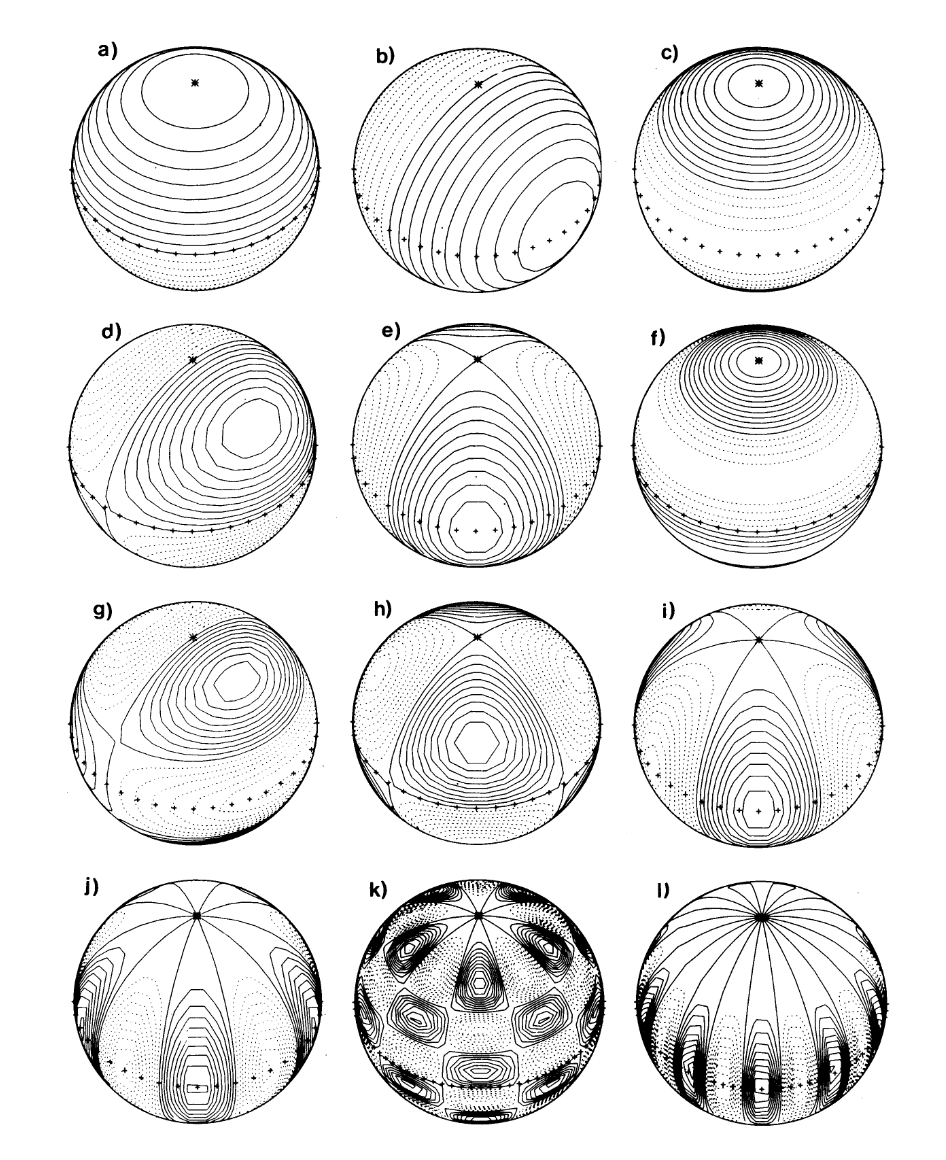
\includegraphics[width=0.9\linewidth]{Imagenes/spherical_harmonics.png}
\caption{Contorno de las partes reales de los armónicos esféricos $Y_m^l$; para simplificar, el factor de fase $(-1)^m$ se ha suprimido. Las líneas de contorno positivas están indicadas por líneas continuas y las negativas por líneas discontinuas. El eje θ = 0 está inclinado en 45º hacia el observador, y se indica con una estrella. El ecuador se muestra como “++++”. Los siguientes casos son ilustrados: a) $l = 1, m = 0$; b) $l = 1, m = 1$; c) $l = 2, m = 0$; d) $l= 2, m = 1$; e) $l = 2, m = 2$; f) $l = 3, m = 0$; g) $l = 3, m = 1$; h) $l = 3, m = 2$; i) $l = 3, m = 3$; j) $l = 5, m = 5$; k) $l = 10, m = 5$; l) $l = 10, m = 10$. Figura tomada de \autocite{ChristensenDalsgaard2019}}
\end{figure}

Al emplear dichos armónicos esféricos como base angular y asumiendo una dependencia temporal armónica de la forma $\exp(-i\omega t)$ (donde $\omega$ es la frecuencia de oscilación propia), podemos escribir las perturbaciones escalares y la componente radial del desplazamiento como:

\begin{align}
\xi_r(r, \theta, \phi, t) &= \sqrt{4\pi}\tilde{\xi}_r(r) Y_l^m(\theta, \phi) \exp(-i\omega t), \\
p'(r, \theta, \phi, t) &= \sqrt{4\pi}\tilde{p}'(r) Y_l^m(\theta, \phi) \exp(-i\omega t),
\end{align}

y de forma análoga para el resto de variables ($\rho', \Phi', \dots$). Las tildes denotan las funciones de amplitud que dependen puramente de la coordenada radial $r$.

Al sustituir estas formas separadas en el sistema de ecuaciones fluido-dinámicas linealizadas derivado en la sección anterior, y recordando que, por la ecuación fundamental que acabamos de resolver, el operador laplaciano horizontal actúa sobre los armónicos esféricos como $\nabla_h^2 Y_l^m = -l(l+1)/r^2 Y_l^m$, podemos dividir todos los términos de las ecuaciones por el factor común $Y_l^m \exp(-i\omega t)$.

Este paso elimina las derivadas angulares y temporales, transformando las ecuaciones en derivadas parciales en un sistema de ecuaciones diferenciales ordinarias (EDOs) unidimensionales para las amplitudes:
\begin{align}
\omega^2 \left[\tilde{\rho}' + \frac{1}{r^2}\frac{d}{dr}(r^2\rho_0\tilde{\xi}_r)\right] &= \frac{l(l+1)}{r^2}(\tilde{p}' + \rho_0\tilde{\Phi}'), \label{eq:1}\\
-\omega^2 \rho_0 \tilde{\xi}_r &= -\frac{d\tilde{p}'}{dr} - \tilde{\rho}'g_0 - \rho_0\frac{d\tilde{\Phi}'}{dr}, \label{eq:2}\\
\frac{1}{r^2}\frac{d}{dr}\left( r^2 \frac{d\tilde{\Phi}'}{dr} \right) - \frac{l(l+1)}{r^2}\tilde{\Phi}' &= 4\pi G \tilde{\rho}', \label{eq:3}
\end{align}

junto con la ecuación de energía adiabática, que se desacopla asumiendo la misma dependencia espacial:
\begin{equation}
(\delta \tilde{p} - \frac{\Gamma_{1,0} p_0}{\rho_0} \delta \tilde{\rho}) = \rho_0(\Gamma_{3,0} - 1)\delta \tilde{q}.
\end{equation}

Como vamos a centrarnos en la aproximación adiabática, el término de ganancia de calor $\delta \tilde{q}$ se anula, simplificando la relación

Es fundamental notar que este sistema depende del grado esférico $l$, pero es totalmente independiente del orden azimutal $m$. Esta degeneración, en la que las frecuencias propias no dependen de $m$, es una consecuencia directa de haber asumido simetría esférica para el estado de equilibrio de la estrella.

\subsection{Oscilaciones Adiabáticas y Condiciones de Contorno}

Para oscilaciones adiabáticas, tenemos que $\delta q = 0$, y podemos reescribir la ecuación de energía como: 

\begin{equation}
    \rho' = \frac{\rho}{\Gamma_1 p} p' + \rho \xi_r \left(\frac{1}{\Gamma_1 p}\frac{dp}{dr} - \frac{1}{\rho}\frac{d\rho}{dr} \right),
\end{equation}

donde hemos suprimido la tilde en las funciones de amplitud y el ``0'' en las cantidades de equilibrio para simplificar la notación. . Este cambio no debería causar confusión.

Podemos utilizar esta ecuación para eliminar $\rho'$ de las ecuaciones \eqref{eq:1} - \eqref{eq:3} y reescribirlas de la siguiente manera:

La ecuación \eqref{eq:1} se convierte en:

\begin{equation}
    \frac{d\xi_r}{dr} = -\left(\frac{2}{r}+\frac{1}{\Gamma_1 p}\frac{dp}{dr}\right)\xi_r + \frac{1}{\rho c^2}\left(\frac{S_l^2}{\omega^2}-1\right) p' + \frac{l(l+1)}{\omega^2 r^2} \Phi',
\end{equation}

donde se introduce la frecuencia acústica característica $S_l$ (o de Lamb) como:
$$S_l^2 = \frac{l(l+1)c^2}{r^2}=k_h^2c^2$$

La ecuación \eqref{eq:2} nos da:
\begin{equation}
    \frac{dp'}{dr} = \rho(\omega^2 - N^2)\xi_r + \frac{1}{\Gamma_1 p}\frac{dp}{dr}p' - \rho \frac{d\Phi'}{dr},
\end{equation}
siendo N la frecuencia de flotabilidad (o de Brunt-Väisälä), dada por:
$$N = g\left(\frac{1}{\Gamma_1 p}\frac{dp}{dr} - \frac{1}{\rho}\frac{d\rho}{dr} \right).$$

Finalmente, la ecuación \eqref{eq:3} se puede escribir como:

\begin{equation}
    \frac{1}{r^2}\frac{d}{dr} \left(r^2\frac{d\Phi'}{dr}\right) = 4\pi G\left( \frac{p'}{c^2} + \frac{\rho \xi_r}{g} N^2\right) + \frac{l(l+1)}{r^2} \Phi'.
\end{equation}

El sistema que acabamos de obtener es un sistema de ecuaciones diferenciales ordinarias de cuarto orden con las variables dependientes $\xi_r$, $\Phi'$, $p'$ y $d\Phi'/dr$. Para que dicho problema esté matemáticamente bien planteado, al tratar con un sistema diferencial de cuarto orden, es imperativo establecer cuatro condiciones de contorno físicas, las cuales pueden encontrarse en la literatura con más detalle:

\begin{itemize}
\item \textbf{En el centro ($r=0$):} Este punto representa una singularidad regular en las ecuaciones. Como es habitual en la teoría de ecuaciones diferenciales, el sistema admite tanto soluciones regulares como singulares en este punto, por lo que dos de las condiciones sirven para seleccionar únicamente las soluciones regulares. Expandiendo las ecuaciones cerca de $r=0$, se demuestra que el desplazamiento $\xi_r$ se comporta como $r^{l-1}$, mientras que $p'$ y $\Phi'$ se comportan como $r^l$. En el caso particular de las oscilaciones radiales, el coeficiente del término de orden principal de $\xi_r$ se anula, de manera que $\xi_r$ es proporcional a $r$. De hecho, por consideraciones geométricas, es evidente que para oscilaciones con simetría esférica el desplazamiento debe anularse en el centro. Además, a partir de estas expansiones, se obtiene que para $l>0$, las soluciones cerca del centro cumplen la relación $\xi_r \simeq l\xi_h$ cuando $r \rightarrow 0$. 

\item \textbf{En la superficie ($r=R$):} Asumiendo que se asigna a la estrella un límite definido en $r=R$, es físicamente razonable suponer que dicha superficie exterior está libre, de modo que no actúan fuerzas sobre ella y el sistema se puede considerar como un sistema aislado. Esto equivale a exigir que la presión sea constante en la superficie perturbada. Por lo tanto, como condición de contorno en la superficie se toma que la perturbación de presión lagrangiana se anule, es decir, $\delta p = p' + \xi_r \frac{dp}{dr} = 0$ en $r=R$. 
Por último, se exige la continuidad de la perturbación del potencial gravitatorio ($\Phi'$) y de su primera derivada en el radio de la superficie ($r=R$). Dado que fuera de la estrella la perturbación de densidad se anula, la ecuación de Poisson puede resolverse de forma analítica. La solución que decae y se anula en el infinito es $\Phi' = A r^{-l-1}$. Como consecuencia, $\Phi'$ debe satisfacer la siguiente condición matemática empalmando con el vacío exterior:
\begin{equation}
    \frac{d\Phi'}{dr} + \frac{l+1}{r}\Phi' = 0 \quad \text{en } r=R.
\end{equation} 
Como información adicional derivada de la condición de la presión, se puede aproximar que la proporción entre el desplazamiento horizontal y radial en la superficie depende únicamente de la frecuencia adimensional ($\sigma$), dada por $\frac{\xi_h(R)}{\xi_r(R)} \approx \sigma^{-2}$.
\end{itemize}
\section{Naturaleza y Clasificación de los Modos de Oscilación}

\subsection{La Aproximación de Cowling} 

Para analizar analíticamente las oscilaciones, a menudo se asume que la perturbación del potencial gravitatorio es despreciable $(\Phi' \approx 0)$. Esta simplificación es válida para grados $l$ grandes o cuando el orden radial $|n|$ es alto. Bajo esta aproximación, el sistema de cuarto orden se reduce a dos ecuaciones diferenciales de primer orden:
\begin{align}
 \frac{d\xi_r}{dr} &= -\left(\frac{2}{r} - \frac{1}{\Gamma_1 H_p}\right)\xi_r + \frac{1}{\rho c^2}\left(\frac{S_l^2}{\omega^2} - 1\right)p' \\
 \frac{dp'}{dr} &= \rho(\omega^2 - N^2)\xi_r - \frac{1}{\Gamma_1 H_p}p',
\end{align}

donde $H_p = -(d \ln p / dr)^{-1}$ es la escala de altura de presión.

\subsection{Frecuencias Características y Atrapamiento} 
Para modos de alto orden radial, las autofunciones varían mucho más rápido que las cantidades de equilibrio. Despreciando las derivadas de estas últimas, el sistema anterior se combina en una única ecuación diferencial de segundo orden que describe el comportamiento local de las ondas: 
$$\frac{d^2\xi_r}{dr^2} = -K(r)\xi_r,$$  

donde la función K(r) viene dada por:
\begin{equation}
    K(r) = \frac{\omega^2}{c^2} \left( \frac{N^2}{\omega^2} - 1 \right) \left( \frac{S_l^2}{\omega^2} - 1 \right)
\end{equation}

La propagación depende de las dos frecuencias características: la frecuencia acústica $(S_l)$ y la de flotabilidad $(N)$. La solución es oscilatoria $(\xi_r \sim \cos(\int K^{1/2} dr + \phi))$ en las regiones de ``atrapamiento'' donde $K(r) > 0$. Fuera de estas regiones $(K(r) < 0)$, la solución decae exponencialmente. Los límites de atrapamiento se sitúan en los puntos de retorno geométricos, donde $K(r) = 0.$

\begin{figure}[htbp]
    \centering
    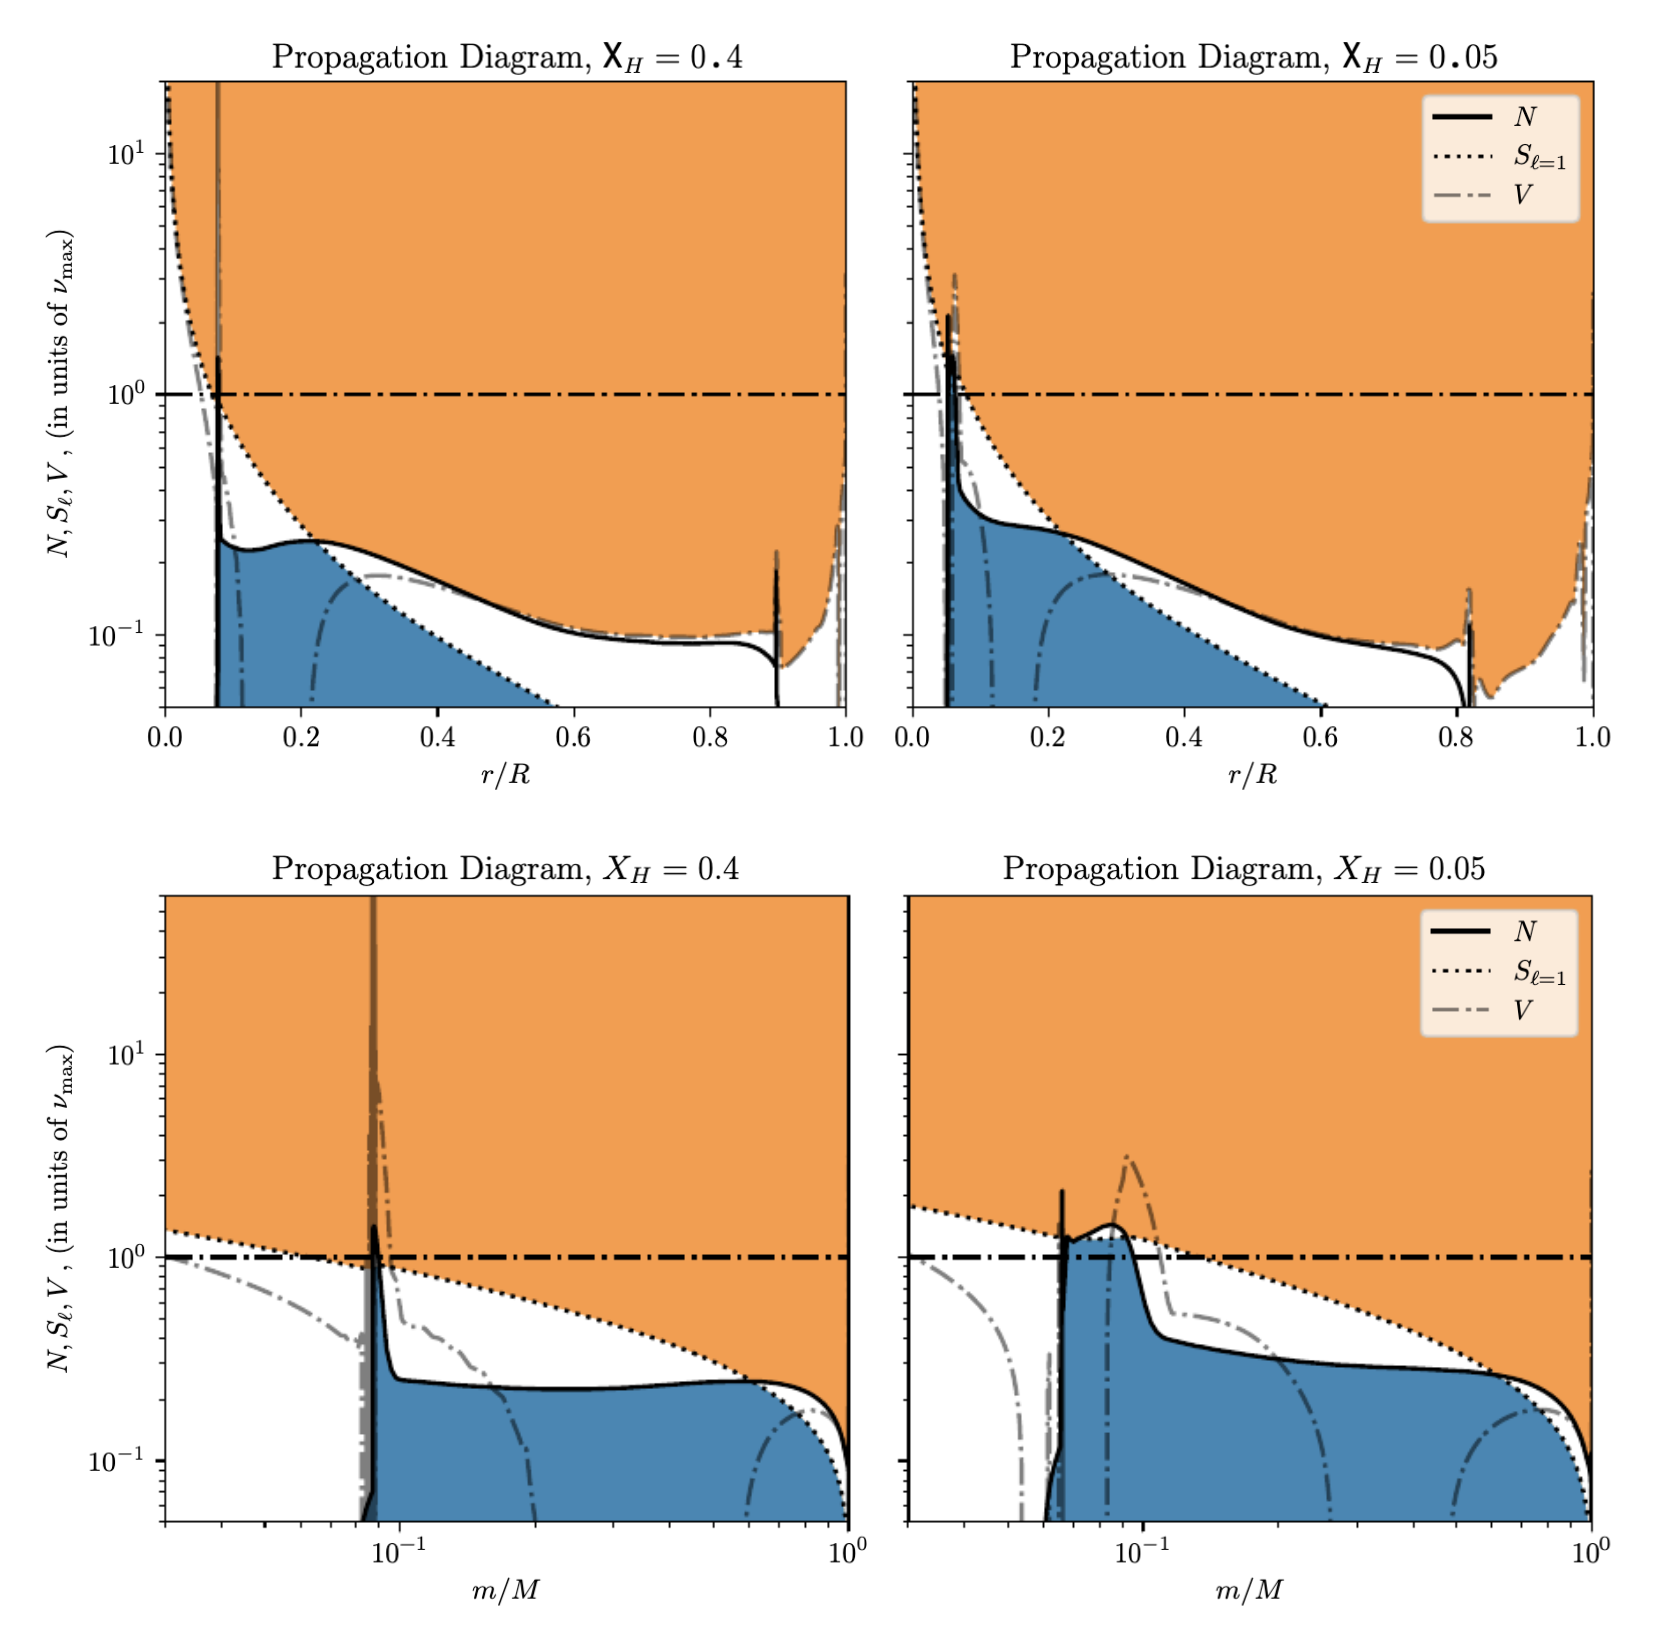
\includegraphics[width=0.9\textwidth]{Imagenes/prop_diagrams.png}
    \caption{Diagrama de propagación para un modelo de $1.4 M_\odot$ con $X_H=0.4$ (línea vertical gris punteada más a la izquierda en Fig. 1) que muestra, en unidades de $\nu_{\text{max}}$, las frecuencias de flotabilidad ($N$), la frecuencia de Lamb ($S_{l=1}$) y el potencial acústico, $V$, que es una frecuencia característica que describe la propagación de los modos radiales de una estrella. La región naranja del diagrama de propagación representa las regiones donde se pueden propagar modos p, mientras que las regiones azules representan las regiones de propagación de modos g. En las capas exteriores de la estrella, la frecuencia mínima a la cual se pueden propagar los modos p está determinada por la frecuencia crítica ($\nu_{\text{crit}}$ imita $V$ cerca de la superficie del modelo) en las capas exteriores. \textbf{Panel superior derecho:} El mismo panel que el anterior pero para el modelo de $1.4 M_\odot$ más tarde en su evolución (línea gris punteada a la derecha en Fig. 1, $X_H=0.05$). \textbf{Paneles inferiores:} Diagrama de propagación para los mismos dos modelos que los superiores, pero el eje x muestra la coordenada relativa de masa en escala logarítmica para mostrar las características cercanas al núcleo en mayor detalle. El potencial acústico, $V$, muestra un pico localizado y agudo en la parte cercana al núcleo.}
    \label{fig:prop_diagrams}
\end{figure}

\subsection{Modos de Presión (p-modes)} 

Corresponden a la rama de altas frecuencias donde $\omega \gg N$. En este límite, la función $K(r)$ se aproxima a:

$$K(r) \simeq \frac{1}{c^2}(\omega^2 - S_l^2)$$

La dinámica está dominada por la velocidad del sonido c (ondas acústicas). La condición del punto de retorno interno $(r_t)$, obtenida al igualar $S_l(r_t) = \omega$, es:

$$\frac{c^2(r_t)}{r_t^2} = \frac{\omega^2}{l(l+1)}$$  

A partir de la relación de dispersión para ondas sonoras planas, el número de onda radial al cuadrado se identifica de forma natural con K:

$$k_r^2 = \frac{1}{c^2}(\omega^2 - S_l^2)$$

En los modos p, la frecuencia de oscilación aumenta con el orden del modo.

\subsection{Modos de Gravedad (g-modes)} 
Corresponden a la rama de bajas frecuencias, encontradas en el interior profundo estelar, donde $\omega^2 \ll S_l^2$. La aproximación para K(r) se convierte en:

$$ K(r) \simeq \frac{1}{\omega^2}(N^2 - \omega^2) \frac{l(l+1)}{r^2} $$

Aquí, la dinámica está controlada por la variación de la frecuencia de flotabilidad $N$, siendo la gravedad la fuerza restauradora sobre las perturbaciones de densidad. Los puntos de retorno vienen dados por la condición $N = \omega$. En congruencia con las ondas de gravedad estacionarias, su número de onda radial es:

$$k_r^2 = \frac{l(l+1)}{r^2}\left(\frac{N^2}{\omega^2} - 1\right)$$

A diferencia de los p-modes, en los modos g el orden aumenta a medida que disminuye $\omega$, y su frecuencia máxima está limitada estrictamente por el valor máximo de $N$ en el interior de la estrella.

\begin{figure}[htbp]
    \centering
    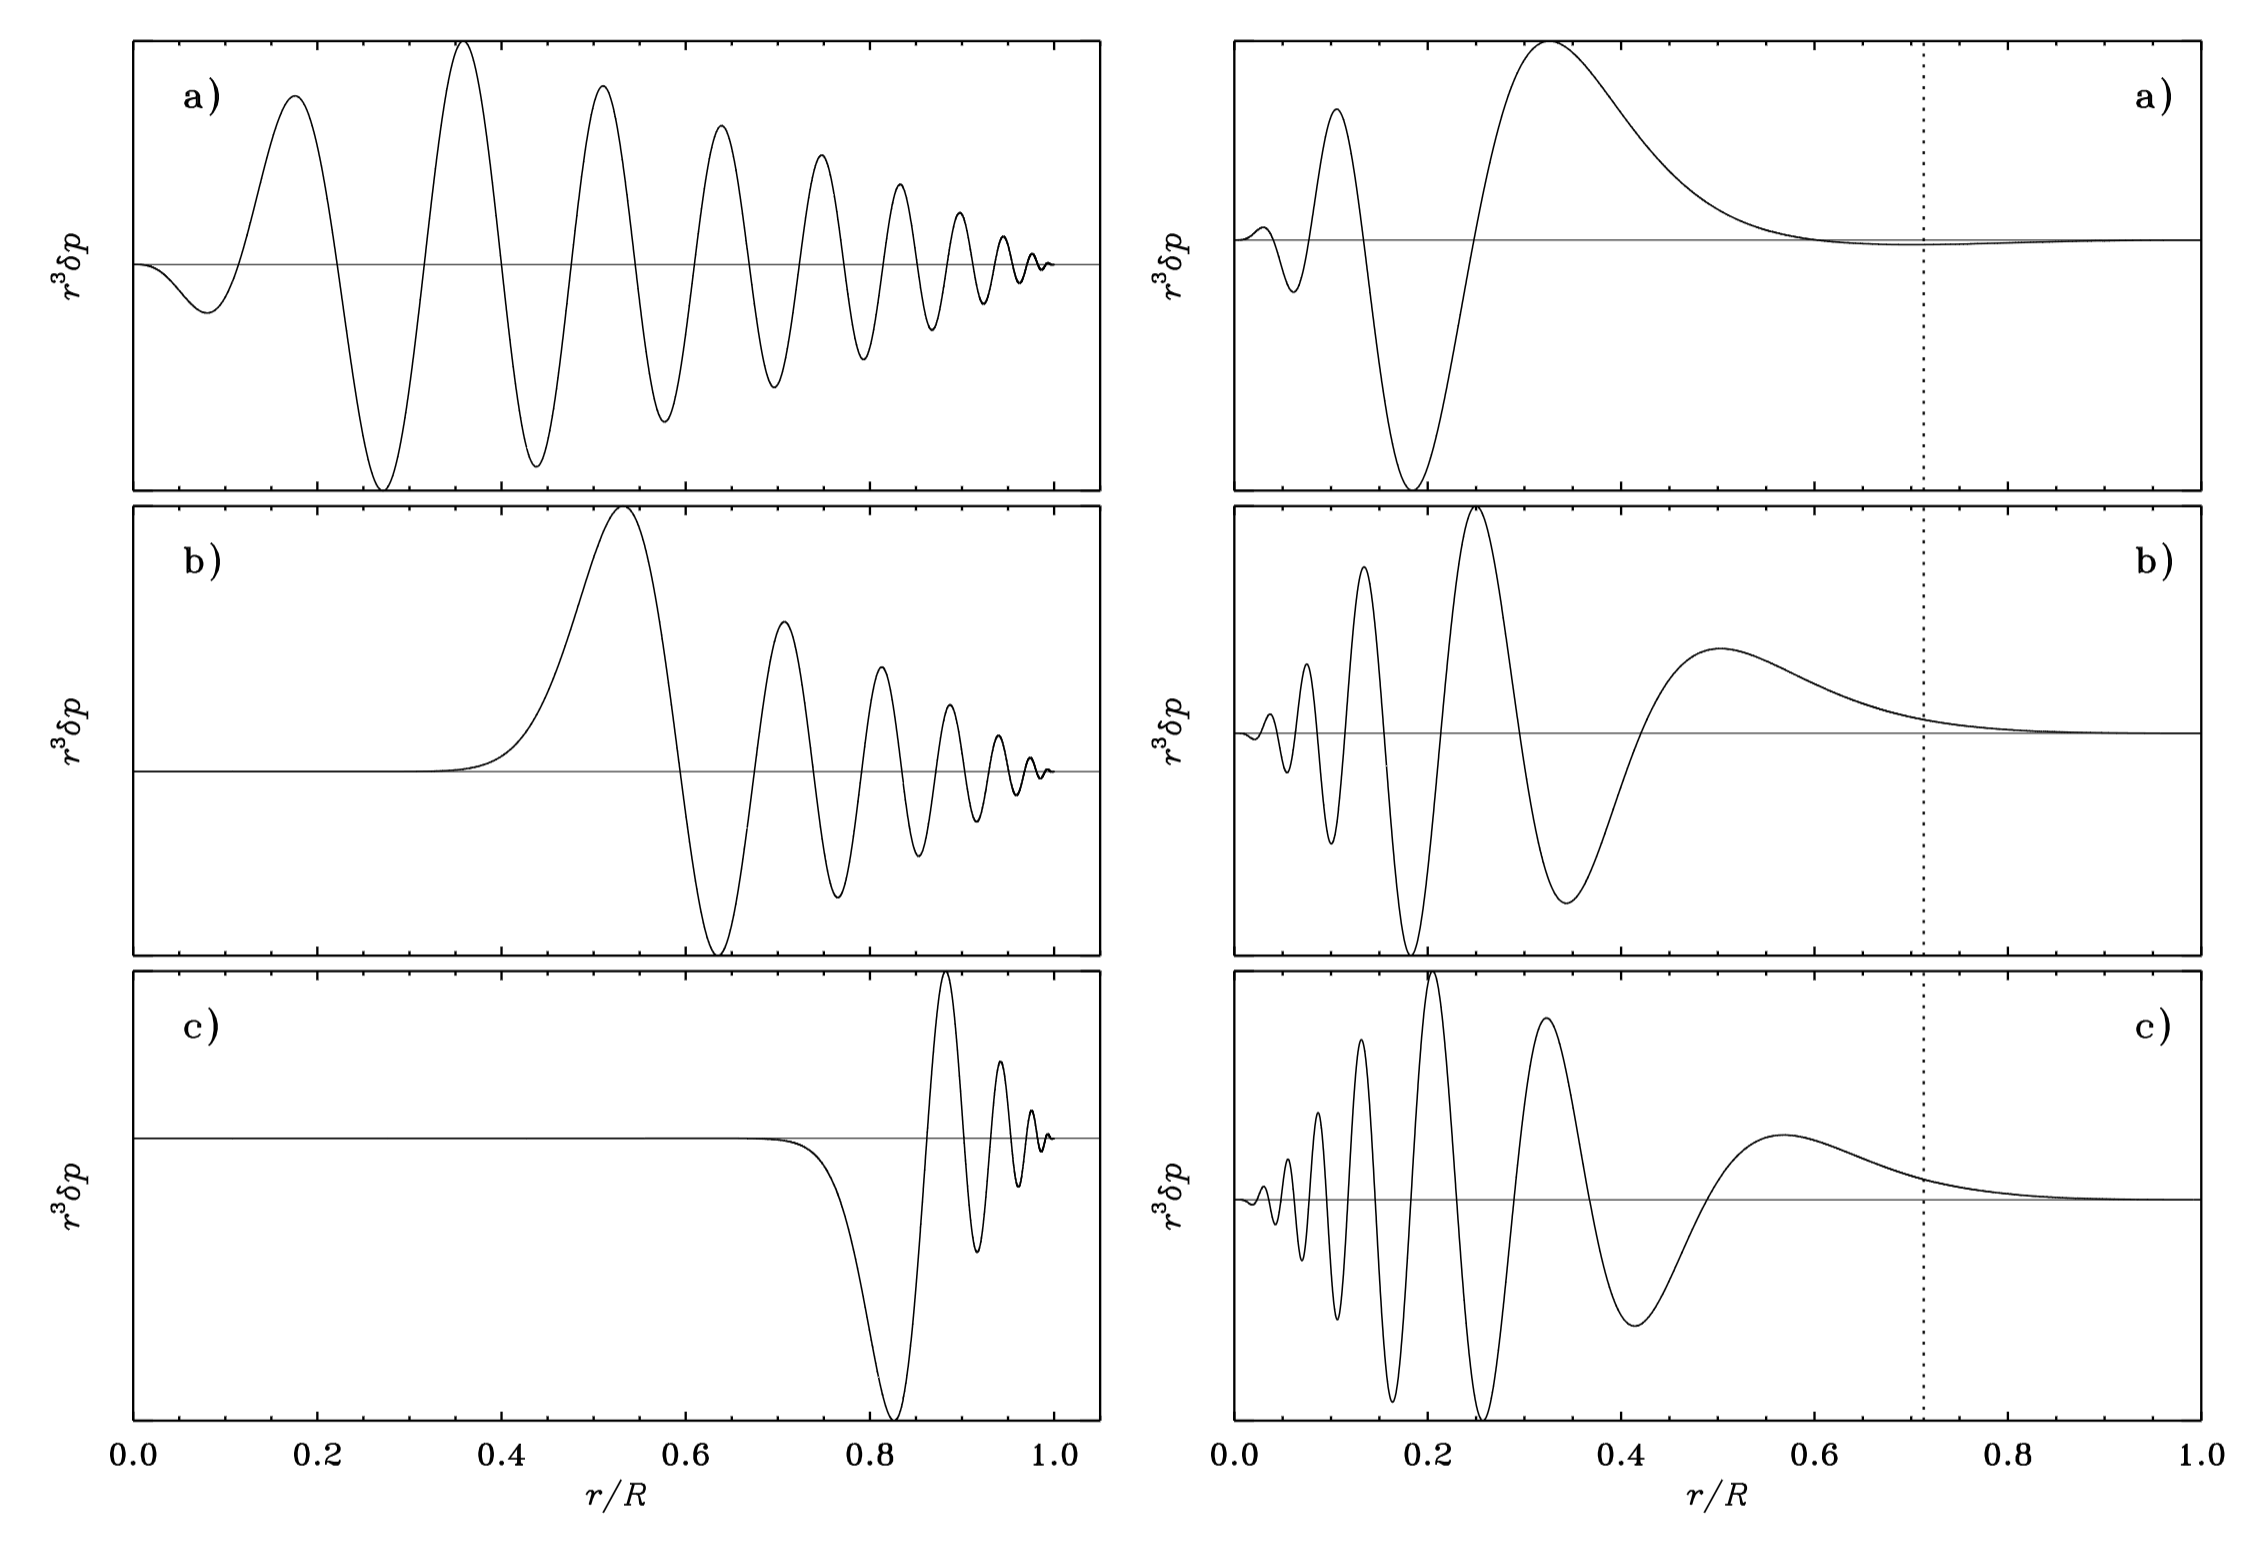
\includegraphics[width=\textwidth]{Imagenes/eigenfunctions.png}
    \caption{Autofunciones normalizadas para un modelo del Sol, en función del radio fraccional. La autofunción elegida, $r^3\delta p$, tiene las dimensiones de energía y está normalizada a su valor máximo. Izquierda: Resultados para 3 modos p: a) ($l = 0, n = 21, \nu = 3038.0\mu$Hz), b) ($l = 20, n = 14, \nu = 2939.2\mu$Hz), y c) ($l = 60, n = 9, \nu = 3043.2\mu$Hz). Derecha: Resultados para 3 modos g: a) ($l = 1, n = -5, \nu = 109.2\mu$Hz), b) ($l = 2, n = -10, \nu = 102.6\mu$Hz), y c) ($l = 3, n = -14, \nu = 104.1\mu$Hz). La línea punteada marca la base de la envoltura convectiva. Imagen tomada de \autocite{Cunha2017}.}
    \label{fig:eigenfunctions_pg_modes}
\end{figure}
